% ---------------------------------------------------------------------------------------------------------------
% This .tex source is an example which *does* use
% the .bib file (from which the .bbl file % is produced).
% REMEMBER HOWEVER: After having produced the .bbl file,
% and prior to final submission, you *NEED* to 'insert'
% your .bbl file into your source .tex file so as to provide
% ONE 'self-contained' source file.
%
% ===============================================================

\documentclass{sig-alternate-05-2015}

%\usepackage{qtree}
\usepackage{listings}
\usepackage[final]{pdfpages}
\usepackage{booktabs}
\usepackage{longtable}
\usepackage{graphicx}

\usepackage{tikz}
\usetikzlibrary{positioning}

% Drasil, short for Yggdrasil.

\newcommand{\lss}{Drasil}
\newcommand{\colAwidth}{0.1\textwidth}
\newcommand{\colBwidth}{0.34\textwidth}

\lstset{language=Haskell}

\begin{document}

% Copyright
\setcopyright{acmcopyright}
%\setcopyright{acmlicensed}
%\setcopyright{rightsretained}
%\setcopyright{usgov}
%\setcopyright{usgovmixed}
%\setcopyright{cagov}
%\setcopyright{cagovmixed}


% DOI
\doi{*******} %D What goes here?

% ISBN
\isbn{978-1-4503-4167-7}

%Conference
\conferenceinfo{SE4Science'16}{Austin, TX, USA}

% \acmPrice{\$15.00}  %D What goes here?

%
% --- Author Metadata here ---
% \conferenceinfo{SE4SC}{2016 ?, ? USA}  %D What goes here?
\CopyrightYear{2016} % Allows default copyright year (20XX) to be over-ridden - IF NEED BE.
%\crdata{0-12345-67-8/90/01}  % Allows default copyright data (0-89791-88-6/97/05) to be over-ridden - IF NEED BE.
% --- End of Author Metadata ---

\title{Position Paper: A Knowledge-Based Approach
to Scientific Software Development
%\titlenote{(Produces the permission block, and
%copyright information). For use with
%SIG-ALTERNATE.CLS. Supported by ACM.}}
%\subtitle{[Extended Abstract]
%\titlenote{A full version of this paper is available as
%\textit{Author's Guide to Preparing ACM SIG Proceedings Using
%\LaTeX$2_\epsilon$\ and BibTeX} at
%\texttt{www.acm.org/eaddress.htm}}
}

\numberofauthors{3} 
\author{
%D No idea what the ordering of this section should be
\alignauthor
Dan Szymczak\\
       \affaddr{McMaster University}\\
       \affaddr{1280 Main Street W}\\
       \affaddr{Hamilton, Ontario}\\
       \email{szymczdm@mcmaster.ca}
\alignauthor
Spencer Smith\\
       \affaddr{McMaster University}\\
       \affaddr{1280 Main Street W}\\
       \affaddr{Hamilton, Ontario}\\
       \email{smiths@mcmaster.ca} 
%D Not sure if you want your email machine-readable
\alignauthor
Jacques Carette\\
       \affaddr{McMaster University}\\
       \affaddr{1280 Main Street W}\\
       \affaddr{Hamilton, Ontario}\\
       \email{carette@mcmaster.ca}
}
\date{}

\maketitle
\begin{abstract}
As a relatively mature field, scientific computing has the opportunity to lead
other software fields by leveraging its solid, existing knowledge base.  By
following a rational design process, desirable software qualities such as
traceability, verifiability, and reproducibility, are arguably easier to reach
than for other classes of software. % <-- Our position is right here

We have begun development of a framework, \lss{}, to put this into practice.
Our aims are to ensure complete traceability, to facilitate agility in the
face of ever changing scientific computing projects, and ensure
that software artifacts can be easily and quickly extracted from \lss{}.
In particular, we are very interested in certifiable software and in
easy re-certification.

Using an example-based approach to our prototype implementation, we have
already seen many benefits. \lss{}
keeps all software artifacts (requirements, design, code, tests, build
scripts, documentation, etc.) synchronized with each other. This allows for
reuse of common concepts across projects, and aids in the verification of
software. It is our hope that \lss{} will lead to the development of higher
quality software at lower cost over the long term.

\end{abstract}


%
%  Use this command to print the description
%
\printccsdesc

\keywords{Literate software, knowledge capture, traceability, software
  engineering, scientific computing, artifact generation.}

\section{Introduction}

We believe that, because of the solid scientific knowledge base built up
over the last $6+$ decades of work in Scientific Computing (SC), it is feasible
for SC to once again take a leadership position as regards the development
of high quality software.  More precisely, our goal is to use this knowledge
to improve the verifiability, reliability, usability, maintainability,
reusability and reproducibility of SC Software (SCS).

Some have argued for a rational document-driven design process 
\cite{SmithAndKoothoor2016}.  However, many researchers have
reported that a document driven process is not used by, nor suitable for, SCS;
they argue that scientific developers naturally use either an agile
philosophy~\cite{CarverEtAl2007, EasterbrookAndJohns2009, Segal2005}, or an
amethododical~\cite{Kelly2013} process, or a knowledge acquisition
driven~\cite{Kelly2015} process.  The arguments are that scientists do not
view rigid, process-heavy approaches favourably~\cite{CarverEtAl2007} and that
in SC, requirements are impossible to determine up-front~\cite{CarverEtAl2007,
  SegalAndMorris2008}.  Rather than abandon the benefits of a rational
document-driven process, we argue that the appropriate tools can in fact
let the scientists focus even more of their time on science.

The principal perceived drawbacks of document-driven design methodologies are:
\begin{itemize}
\setlength{\itemsep}{0.0em}
\setlength{\parskip}{0pt}
\setlength{\parsep}{0pt}
\item information duplication,
\item synchronization headaches between artifacts,
\item an over-emphasis on non-executable artifacts.
\end{itemize}

Thus, we argue that successfully achieving our goal of improving various
software qualities (verifiability, reliability, usability, etc.) of SCS, whilst
also improving, or at least not diminishing performance, requires that we find a
way to simultaneously deal with the above drawbacks. In fact, we are more
ambitious: we want to improve developer productivity and thus save time and
money on SCS development, certification and re-certification. To accomplish this
we need to remove duplication between software artifacts \cite{WilsonEtAl2013}
as well as provide traceability between all software artifacts. In practice,
this means providing facilities for automatic software artifact generation from
high level ``knowledge.'' We can accomplish this by having a single ``source''
for each relevant piece of information which makes up an SC problem and its
solution. From this, we can generate all required documents and views. That is,
we aim to provide methods, tools and techniques to support a literate process
for developing scientific software that generalizes the idea behind
Knuth's~\cite{Knuth1984} literate programming. Unlike other document generation
tools, like Doxygen, the focus is on all software artifacts, not just the code
and its comments.

%D May need to cut the roadmap for space.
In the following section, we  
%Section~\ref{sec:background} will give a more in-depth 
focus on SCS quality and literate programming.
%Section~\ref{sec:lss} 
Then we introduce our framework, \lss{}.  We show
a short example of the framework and discuss its advantages. 
%Section~\ref{sec:todo} will discuss
We then discuss how we want the framework to evolve. % and what future work we
%intend to do. %Finally, Section~\ref{sec:conclusion}  
The last section provides concluding remarks.

\section{Background} \label{sec:background}

In this section we discuss challenges for developing SCS and we
introduce the ideas behind our approach.

\subsection{Challenges} \label{ssec:challenges}

As the best numerical approach to solve a given problem is usually not known a
priori, we have to face the \textit{technique selection
  challenge}~\cite{Yu2011}. Experimentation is inevitably necessary to determine
the appropriate order of interpolation, the degree of implicitness,
etc. Nevertheless, the problem to solve does not change.  This implies that we
need a separation of concerns between the physical model and the numerical
algorithms.  Ease of experimentation means that we also need facilities to
parameterize algorithmic variabilities.

In an effort to make scientific libraries and software as widely applicable as
possible, most packages provide a generic interface with a large number of
options; this tends to overwhelm users and cause programmers to not reuse
libraries, since they do not believe the interface needs to be as complicated
as it appears~\cite{Dubois2002}. This is the \textit{understandability}
challenge~\cite{Yu2011}.  An ideal framework would expose an
API, as well as generate applications, which use routines which are only as
complicated as they need to be for the job at hand.

As requirements change, we face the \textit{maintainability
challenge}~\cite{Yu2011}.  The high frequency of change for SCS
causes accute problems for certification. If the expense and time required for
re-certification is on the same order of magnitude as the original
certification, changes will not be made. To be effective in this environment, a
framework needs to provide traceability, so the consequences of change can be
directly evaluated.

\subsection{Literate Programming} \label{ssec:literate}

Literate programming (LP) is a methodology introduced by Knuth
\cite{Knuth1984}. The main idea is to write programs in a way that explains 
{\bf (to humans)} what we want the computer to do, as opposed to simply giving
the computer instructions.

In a literate program, the documentation and code are together in one source.
While developing a literate program, the algorithms used are broken down into
small, understandable parts (known as ``sections'' \cite{Knuth1984} or
``chunks'' \cite{JohnsonAndJohnson1997}) which are explained, documented, and
implemented in an order which promotes understanding. To get working source
code, the \textit{tangle} process is run, which extracts the code from the
literate document and reorders it into an appropriate structure acceptable
to one's compiler.  Similarly, the \textit{weave} process is run to extract and
typeset the documentation.
There are several examples of SC programs being written in LP style, such as
VNODE-LP \cite{Nedialkov2006} and ``Physically Based Rendering: From Theory to
Implementation'' \cite{PharrAndHumphreys2004} (a literate program which is also
a successful textbook!).

\begin{figure}
%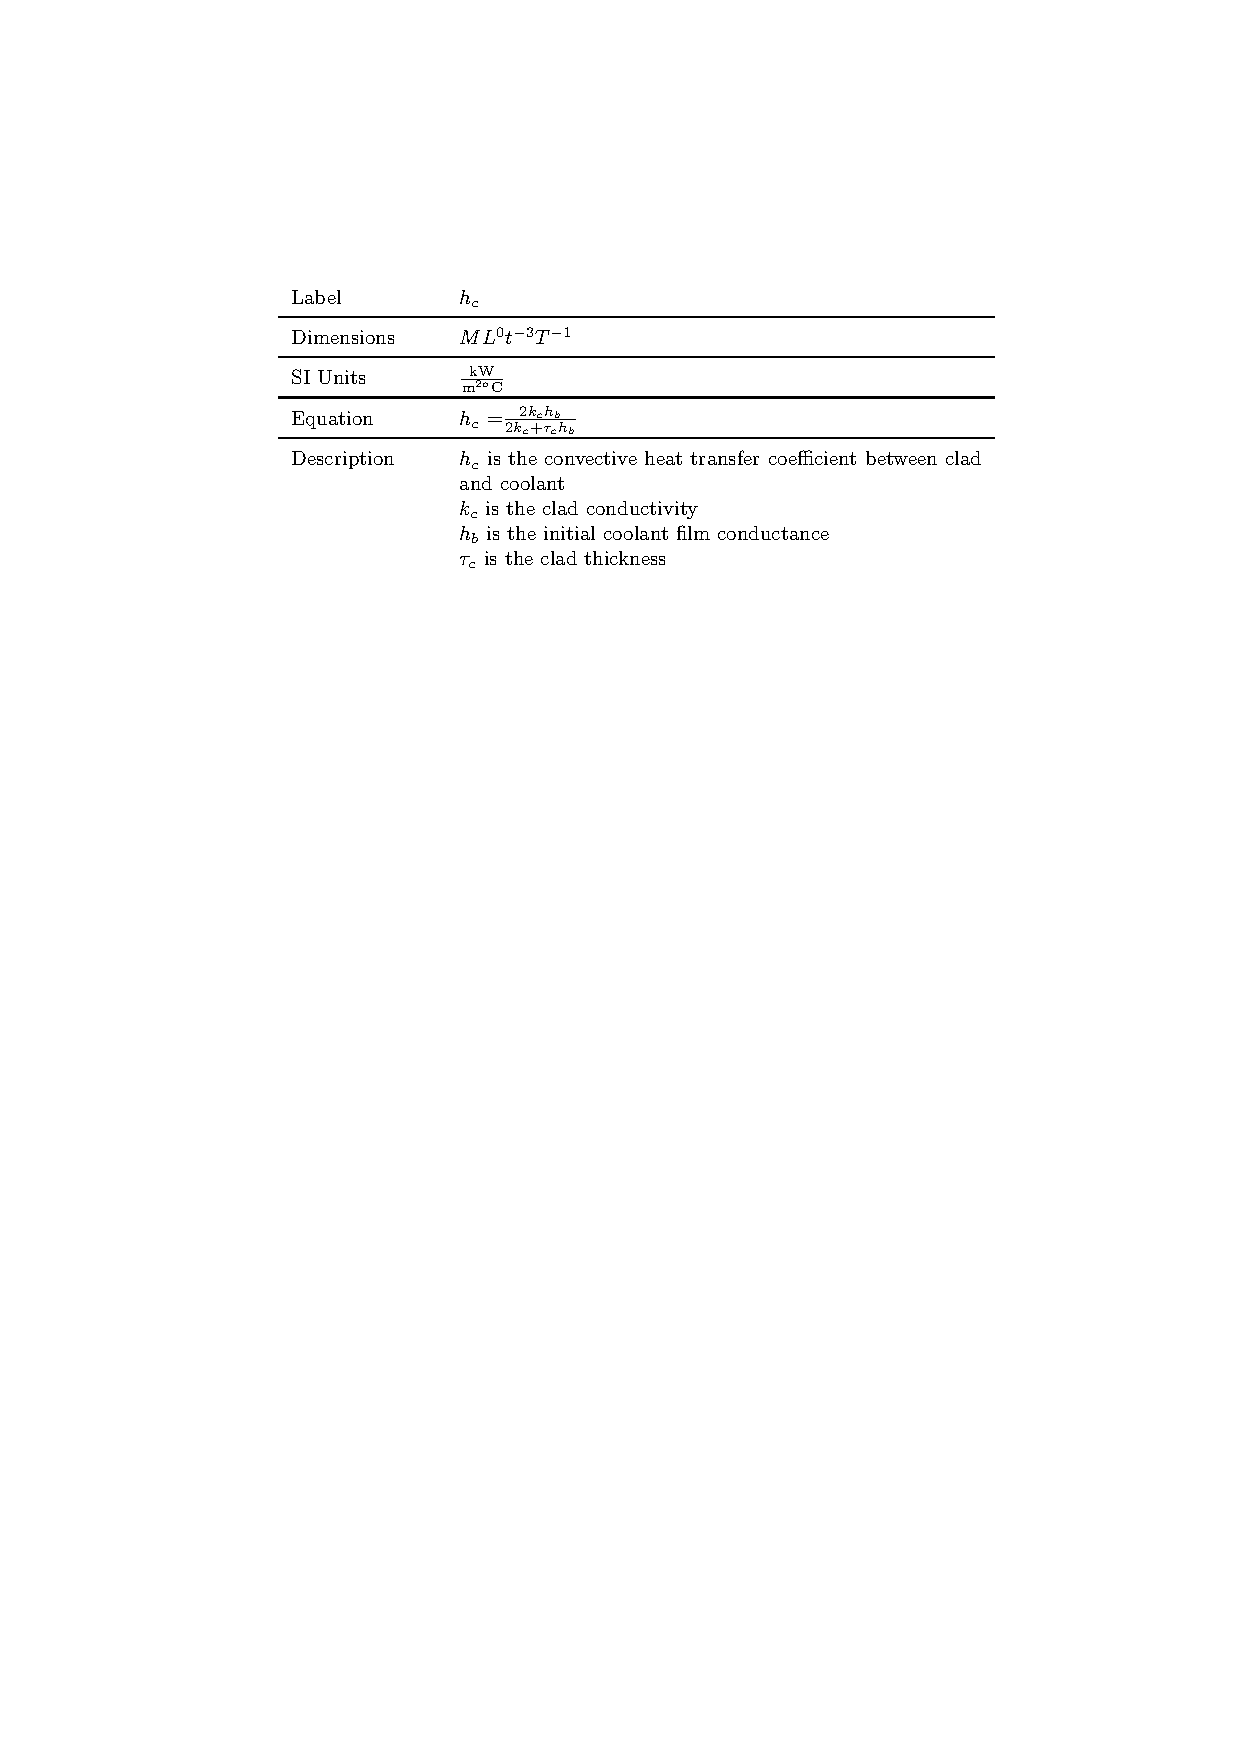
\includegraphics[width=0.49\textwidth]{h_c.pdf}
~\newline \noindent \begin{minipage}{\textwidth}
\begin{tabular}{p{\colAwidth} p{\colBwidth}}
%\toprule \textbf{Number} & \textbf{DD\refstepcounter{datadefnum}\thedatadefnum \label{hc}}
%\\ \midrule 
Label & 
$h_{c}$
\\ \midrule
Dimensions & $ML^0t^{-3}T^{-1}$\\ \midrule
SI Units & $\mathrm{\frac{kW}{m^{2o}C}}$\\ \midrule
Equation & $h_{c}$ =$
\frac{2k_{c}h_{b}}{2k_{c}+\tau_{c}h_{b}}$\\ \midrule
Description &  $h_{c}$ is the convective heat transfer coefficient between clad and coolant
\newline
$k_{c}$ is the
clad conductivity \newline
$h_{b}$ is the
initial coolant film conductance \newline
$\tau_{c}$ is the
clad thickness 
\newline
%NOTE: Equation taken from the code\\ \midrule  Sources & source code \\ \bottomrule 
\end{tabular} \end{minipage}\\ 
\caption{SRS data definition of $h_c$}
\label{fig:h_c}
\end{figure}	

\section{Introducing \lss} \label{sec:lss}

In \lss, we accomplish our two primary objectives (complete traceability, and
eliminating knowledge duplication) by generalizing the literate approach.

\subsection{A Simple Example} \label{ssec:example}

We have used a practical, example-driven approach to the development of \lss{}.
Our first example involves 
the simplified Software Requirements Specification (SRS) for a fuel pin in a
nuclear reactor (see \cite{SmithAndKoothoor2016} for more details). To get
started, let us look specifically at the term $h_c$ (defined in
Figure~\ref{fig:h_c}).  This defines a concept, its units, its
defining equation, and the description of the other concepts upon which it
depends.

We can currently generate the \verb|.tex| file for
much of the SRS for the fuel pin as well as the source code (in C) for the
required calculations.

\subsection{Design} \label{sssec:ex_how}

The fundamental task for \lss{} is \emph{knowledge capture}, in such a 
way that this knowledge can be viewed in different ways (code, specification,
etc).  Each individual piece of knowledge is a named \textit{chunk}; putting
chunks together is done via a \textit{recipe}; a \textit{generator} then
interprets recipes to produce the desired view.  

\begin{figure}
\begin{center}
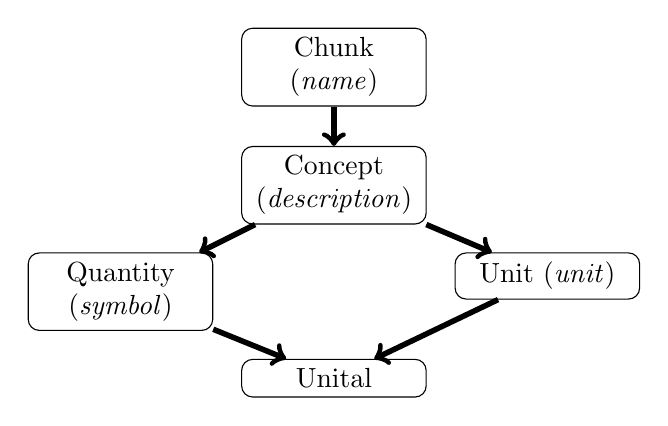
\begin{tikzpicture}[node distance=5mm]
  \tikzstyle{every node}=[draw,shape=rectangle, rounded corners,
    text width=6em, text centered];
  \node (ch)                     {Chunk (\emph{name})};
  \node (co) [below = of ch]       {Concept (\emph{description})};
  \node (qu) [below left = of co]  {Quantity (\emph{symbol})};
  \node (u ) [below right = of co] {Unit (\emph{unit})};
  \node (uc) [below right = of qu] {Unital};

  \draw [->, line width=2pt] (ch) -- (co);
  \draw [->, line width=2pt] (co) -- (qu);
  \draw [->, line width=2pt] (co) -- (u );
  \draw [->, line width=2pt] (qu) -- (uc);
  \draw [->, line width=2pt] (u ) -- (uc);
\end{tikzpicture}
\end{center}
%\begin{center}
%{
% 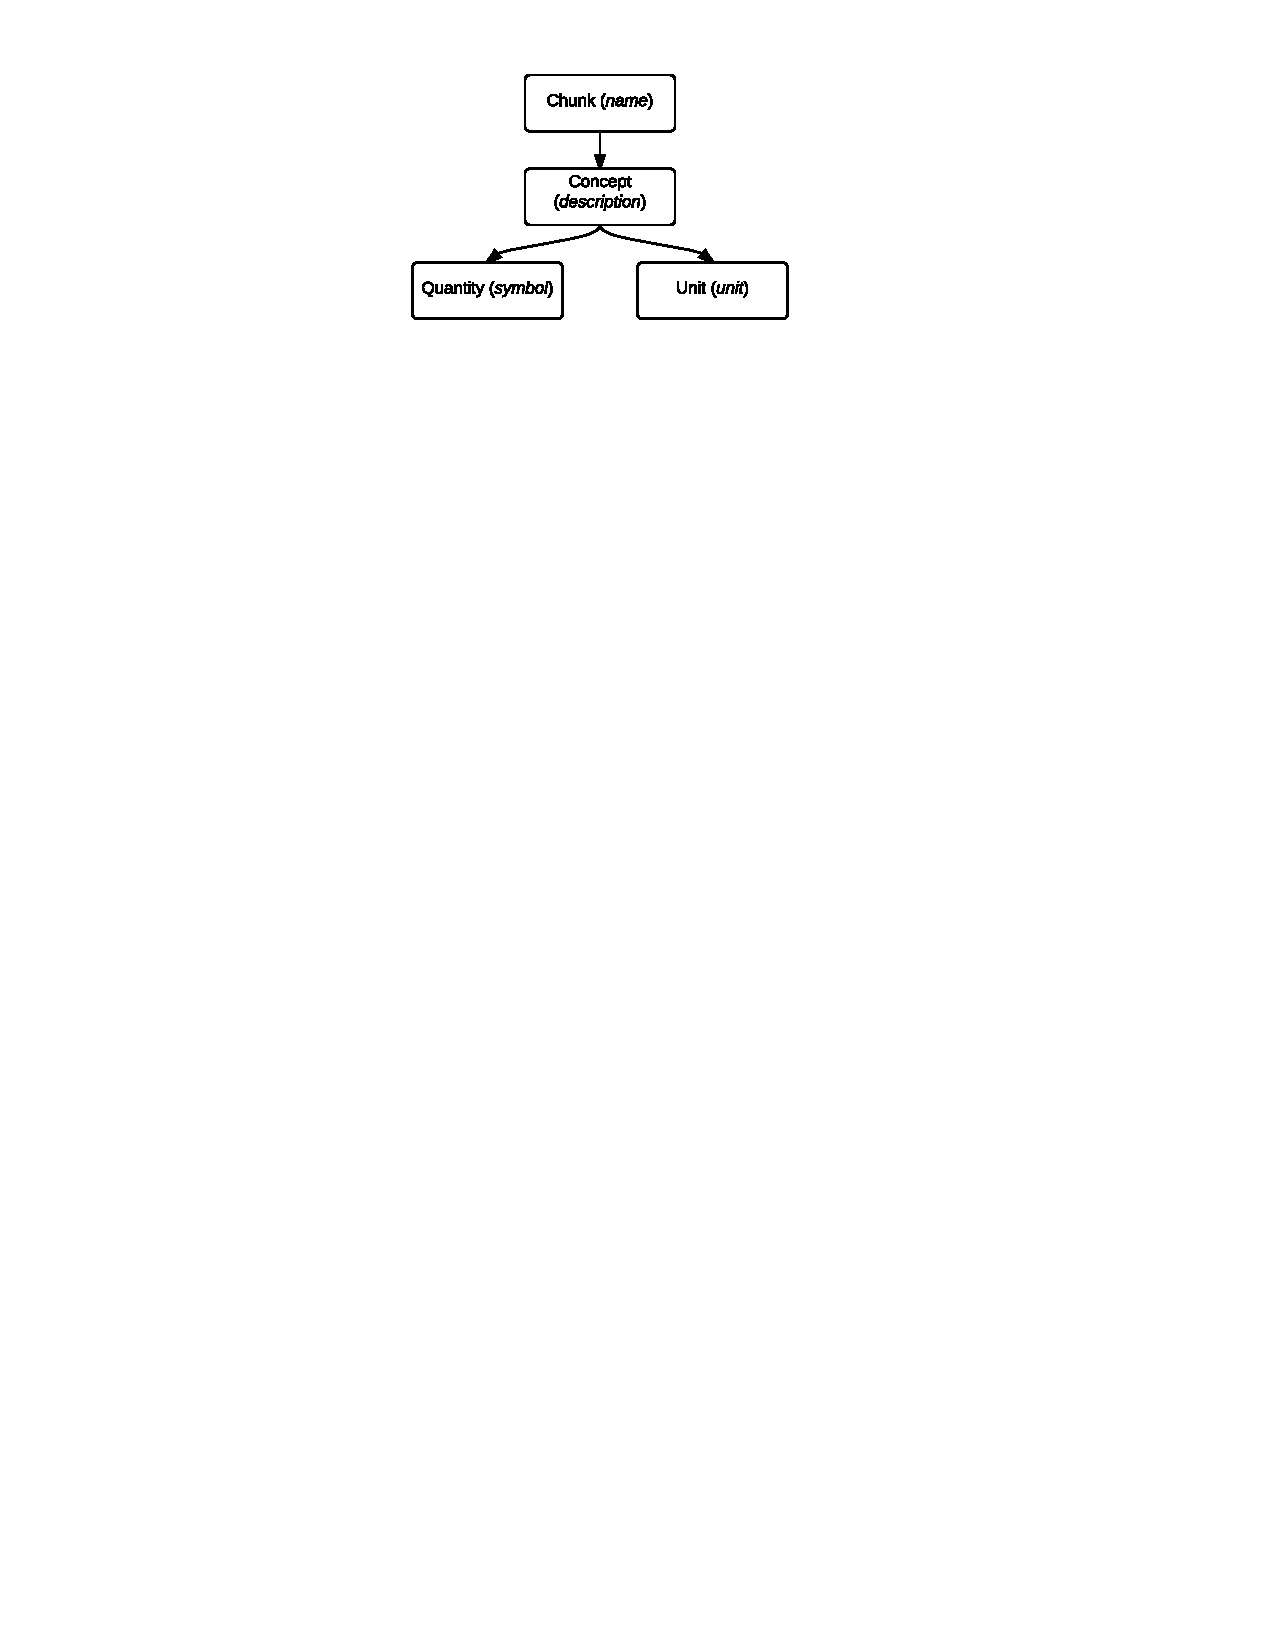
\includegraphics[width=0.35\textwidth]{ChunkHierarchy.pdf}
%}
%\end{center}
\caption{The chunk design}
\label{fig:chunks}
\end{figure}

We have different kinds of chunks.  The most basic ones are simply named pieces
of information.  Most however represent some \emph{concept}, which has a
\emph{description}.  In the SC context, many concepts are \emph{quantities},
which are represented by a specific \emph{symbol}.  Orthogonally, a \emph{unit}
is also a concept.  Most quantities have units.  And so on (as pictured
in Fig.~\ref{fig:chunks}).

By breaking things down in this way, we can assemble most concepts from
pre-existing chunks -- see Fig.~\ref{fig:recipe} for an SRS recipe that
uses (among other things) $h_c$. %D ``among others removed for brevity''?

\begin{figure}[tb]
\begin{lstlisting}[frame=single, 
  showstringspaces=false, basicstyle=\scriptsize]
srsBody = srs [h_g, h_c] "Spencer Smith" [s1,s2]

s1 = Section (S "Table of Units") [intro, table]

table = Table 
 [S "Symbol", S "Description"] (mkTable
   [(\x -> Sy (x ^. unit)),
    (\x -> S (x ^. descr)) ] si_units)

intro = Paragraph (S "Throughout this ...")
\end{lstlisting}
\caption{A portion of the SRS recipe}
\label{fig:recipe}
\end{figure}

Currently, recipes are specified using a collection of DSLs embedded in
Haskell.  We have a DSL for expressions, expression layout, document
layout, C code, and LaTeX code.  For example, the expression layout DSL
describes how expressions should appear (subscript and
superscripts, concatenation of symbols, etc.), whereas the document layout
DSL deals with sections, tables, etc.

We have broken down our example into common knowledge, specific knowledge
and a recipe for an SRS (see Figure~\ref{fig:recipe}).
Here the fundamental SI units are common knowledge. Each is
contained within its own chunk in the SI unit library -- see
Figure~\ref{fig:know_common} for a taste.

\begin{figure}[thb]
\begin{lstlisting}[frame=single, showstringspaces=false, 
  basicstyle=\scriptsize]
metre, second, kelvin :: FundUnit
metre  = fund "Metre"  "length (metre)"       "m"
second = fund "Second" "time (second)"        "s"
kelvin = fund "Kelvin" "temperature (kelvin)" "K"
\end{lstlisting}
%mole   = fund "Mole"   "amount of substance (mole)"   "mol"
%kilogram = fund "Kilogram" "mass (kilogram)"      "kg"
%ampere   = fund "Ampere"   "electric current (ampere)"    "A"
%candela  = fund "Candela"  "luminous intensity (candela)" "cd"
\caption{Segment of the SI unit library}
\label{fig:know_common}
\end{figure}

The $h_c$ chunk (Figure~\ref{fig:know_specific}) is specific
knowledge: it contains the name, description, symbol, units, and equation
for $h_c$.

\begin{figure}
\begin{lstlisting}[frame=single, showstringspaces=false, basicstyle=\small]
h_c_eq :: Expr
h_c_eq = 2*(C k_c)*(C h_b) /
  (2*(C k_c) + (C tau_c)*(C h_b))

h_c :: EqChunk
h_c = fromEqn "h_c" 
 "convective heat transfer coefficient between 
    clad and coolant"
   (sub h c) heat_transfer h_c_eq
\end{lstlisting}
\caption{The $h_c$ chunk}
\label{fig:know_specific}
\end{figure}

The internal expression language \lstinline|Expr|
allows for the straighforward generation of source code. We utilize methods
similar to those found in \cite{SAGA:DSL, Szymczak2014}
wherein the expression language is converted to an abstract representation of
the code and then passed to a pretty-printer to create the final source.

We currently generate C code, however it would be possible to generate any
language provided we have an appropriate representation for that language.

\subsection{Advantages} \label{ssec:advantages}

We can already see some advantages over traditional SC
development. How \lss{} addresses the specific challenges of
Section~\ref{ssec:challenges} will be explored below.

\subsubsection{Knowledge Capture} \label{sssec:adv_knowledge}

At the appropriate abstraction level, many SC problems have significant
commonality, since a large class of physical models are instances of a
relatively small number of conservation equations (conservation of energy, mass
and momentum).  For instance, the theoretical model for conservation of thermal
energy for a fuel pin in \cite{SmithAndKoothoor2016} is written generally, without
reference to a specific coordinate system.  The exact same theoretical model can
be reused in any thermal model.  The variation in the final instanced model will
come from the refinement of the theory using assumptions appropriate to the
problem.

Our approach aims to build libraries of knowledge that can be reused anywhere.
Each library should contain common chunks relevant to a specific application
domain (ex. thermal analysis) and each project should aim to reuse as much as
possible during development.

From our example, a common source of reused knowledge is the 
\emph{Syst\`{e}me international d'unit\'{e}s}, also known as
SI units (Figure~\ref{fig:know_common}). They are commonly
used throughout all of SC, so why should they be redefined for each
project? Once the knowledge has been captured, it can simply be reused.
With \lss{} this is possible with minimal effort, allowing developers and
scientists to spend their valuable time on more important tasks.

\subsubsection{Software Certification} \label{sssec:adv_cert}

Current software certification processes require high-quality documentation.
Depending on the regulatory body and the certification standards, many types of
documents may be required, such as the requirements specification, verification
plans, design specification and code. However, creating these should not impede
a scientist's work. As requirements and numerical algorithmic decisions change,
documentation and code must be updated. This creates issues with traceability
and maintainability. \lss{} aims to generate these documents alongside the code,
while accounting for any changes. When properly used, singular knowledge will be
embodied in a single chunk, and the generation process will take care of baking
this information into all appropriate places in the documentation and code. Thus
any change is guaranteed to propagate throughout all of the artifacts.

Recipes are useful too: if a document standard were to be changed during the
development cycle, it would not necessitate re-writing the entire document. All
of the information in the chunks would remain intact, only the recipe would need
to be changed to accommodate the new view. Traceability has the advantage
of also improving reproducibility.

%D This next section really feels like it's making a promise without really
%  explaining how/why it'll work.
\subsubsection{"Everything should be made as simple as possible, but not
  simpler."  --- Einstein} \label{sssec:adv_simple}

Take finite element methods as one example:  while there exist many powerful,
general commercial programs for this, they are not often used to
develop new ``widgets'' because they are hard to understand.  Thus
engineers often resort to building and testing prototypes, instead of
performing simulations, due to a lack of clearly relevant tools.

By using recipes that generate versions of general algorithms specific to
a particular problem, we can generate applications suited to the needs of
the engineers.  Changes in specifications can be reflected in the code in
(essentially) real-time at trivial cost. For example, if an engineer were
designing parts for strength, they could start from a general stress analysis
knowledge base.  This could then be specialized to (say) plane stress/strain,
depending on which assumption would be most appropriate at the time. The
generated program could even be customized to the parameterized shape of
the part the engineer is interested in.  %  Importantly, the generated program
% can be generated to only expose the degrees of freedom necessary for the
% engineer to change (ex. material properties or specific dimensions of the
% part), making the simulation process simpler and safer.
Importantly, the simulation process is made simpler because an engineer is not
required to interact with the source code; they simply modify those degrees of
freedom (ex. material properties or specific dimensions of the part), that are
exposed to them by the generator.

\subsubsection{Verification} \label{sssec:adv_verify}

When it comes to verification, requirements documents typically include
so-called ``sanity'' checks (see $2^{\text{nd}}$ column of Table~\ref{tab:pcm})
that can be reused throughout subsequent phases of development. For instance, a
requirement could assume conservation of mass or constrain lengths to be always
positive. The former would be used to test the output and the latter to guard
against invalid inputs.

\begin{table} 
\centering
\caption{Constraints on quantities}
\begin{tabular}{|c|c|r|c|} \hline
\textbf{Var} & \textbf{Constraints} & \textbf{Typical Value} & \textbf{Uncertainty}\\ \hline
$L$ & $L > 0$ & 1.5 m & 10\% \\ \hline
$D$ & $D > 0$ & 0.412 m & 10\% \\ \hline
$V_P$ & $V_P > 0$ & 0.05 m$^3$	& 10\% \\ \hline
$A_P$ & $A_P > 0$ & 1.2 m$^2$	& 10\% \\ \hline
$\rho_P$ & $\rho_P > 0$	& 1007 kg/m$^3$	& 10\% \\
\hline\end{tabular}
\label{tab:pcm}
\end{table}

With \lss, these sanity checks can also be captured and re-used.  Each chunk
can maintain its own sanity checks (as constraints) and recipes can incorporate
them into generated systems, either for testing or for in-field use, to ensure
all inputs and outputs (including intermediaries) are valid.

Through recipes, complete traceability is achievable: as knowledge must be
drawn together explicitly, one can automatically list all chunks that were
used by a recipe.

Finally, because all knowledge has a unique source, any mistakes that occur in
the generated software artifacts will occur \textbf{everywhere}. Errors
propagate through artifacts, and the artifacts will always be in sync with each
other (and the source). As a consequence, errors will be much easier to see,
and thus easier to find and fix.  

\section{Future work} \label{sec:todo}

Our prototype is still in its early stages, producing only one document type
(the SRS) and only one type of code (C code for calculations), but has 
already been a great source of inspiration to us. We plan to expand
\lss{} in several ways, including at least:
\begin{enumerate}
\setlength{\itemsep}{0pt}
\setlength{\parskip}{0pt}
\setlength{\parsep}{0pt}
\item Generate more artifact types. %(i.e. have more default recipes).
\item Generate different document views. %(ex. SRS with equation derivations).
\item More types of information in chunks (see Table~\ref{tab:pcm}).
\item Use these constraints to generate test cases.
\item Implement much larger examples.
\end{enumerate}

For the generation of test cases, physical constraints will be seen as hard
limits on values (ex. length must always be positive and a negative value would
throw an error). Typical values, on the other hand, are ``reasonable'' values
(ex. the length of a beam should be on the order of several metres, but
theoretically it could be kilometres, thus the code will raise a warning
instead of an error).

\section{Concluding Remarks} \label{sec:conclusion}

The development of high-quality SCS, especially those which can be
(re-)certified, leave much to be desired.  The burden of keeping documentation
and code synchronized, due to hand-duplicated information, leads to many 
problems.  The end result tends to involve either extremely high development
costs (and bored developers), or software of dubious quality which is 
difficult to maintain.

Our position is that desirable software qualities such as
traceability, verifiability, and reproducibility can be achieved for SCS and in the future we hope to show this using \lss{}.
%With \lss{}, we hope to achieve complete traceability between all software
%artifacts, while causing as little inconvenience to the developers as possible.
We hope that this will lead to higher quality software, at a lower
\emph{long term} cost.

\bibliographystyle{abbrv}
\bibliography{drasil}  
\end{document}
